\documentclass{scrartcl}
\usepackage{german}
\usepackage[utf8]{inputenc}
\usepackage[german]{babel}

% zusätzliche mathematische Symbole, AMS=American Mathematical Society
\usepackage{amssymb}
\usepackage{amsmath}
% fürs Einbinden von Graphiken
\usepackage{graphicx}
\usepackage{verbatim}

% für Namen etc. in Kopf- oder Fußzeile
\usepackage{fancyhdr}

% erlaubt benutzerdefinierte Kopfzeilen
\pagestyle{fancy}

% um tabelle nach links zu schieben
\usepackage{changepage}

% Definition der Kopfzeile
\lhead{
\begin{tabular}{lllll}
Nils Hagner & 4346038 & Felix Karg & 4342014 \\
Michael Fleig & 4340085 & Anush Davtyan &4368689
\end{tabular}
}
\chead{}
\rhead{\today{}}
\lfoot{}
\cfoot{Seite \thepage}
\rfoot{}

\begin{document}

\section*{Solutions for Excercise sheet 3}

\subsection*{Exercise 1 – Requirements Elicitation}
\begin{itemize}
    \item[i] Explicitly different situations represented in the following questions. \\
    \item[ii]
        \verbatiminput{questions.txt}
        Before, those interpretations seemed all plausible:
        \verbatiminput{interpretations.txt}
\end{itemize}



\subsection*{Exercise 2 – Analysis of Decision Tables}

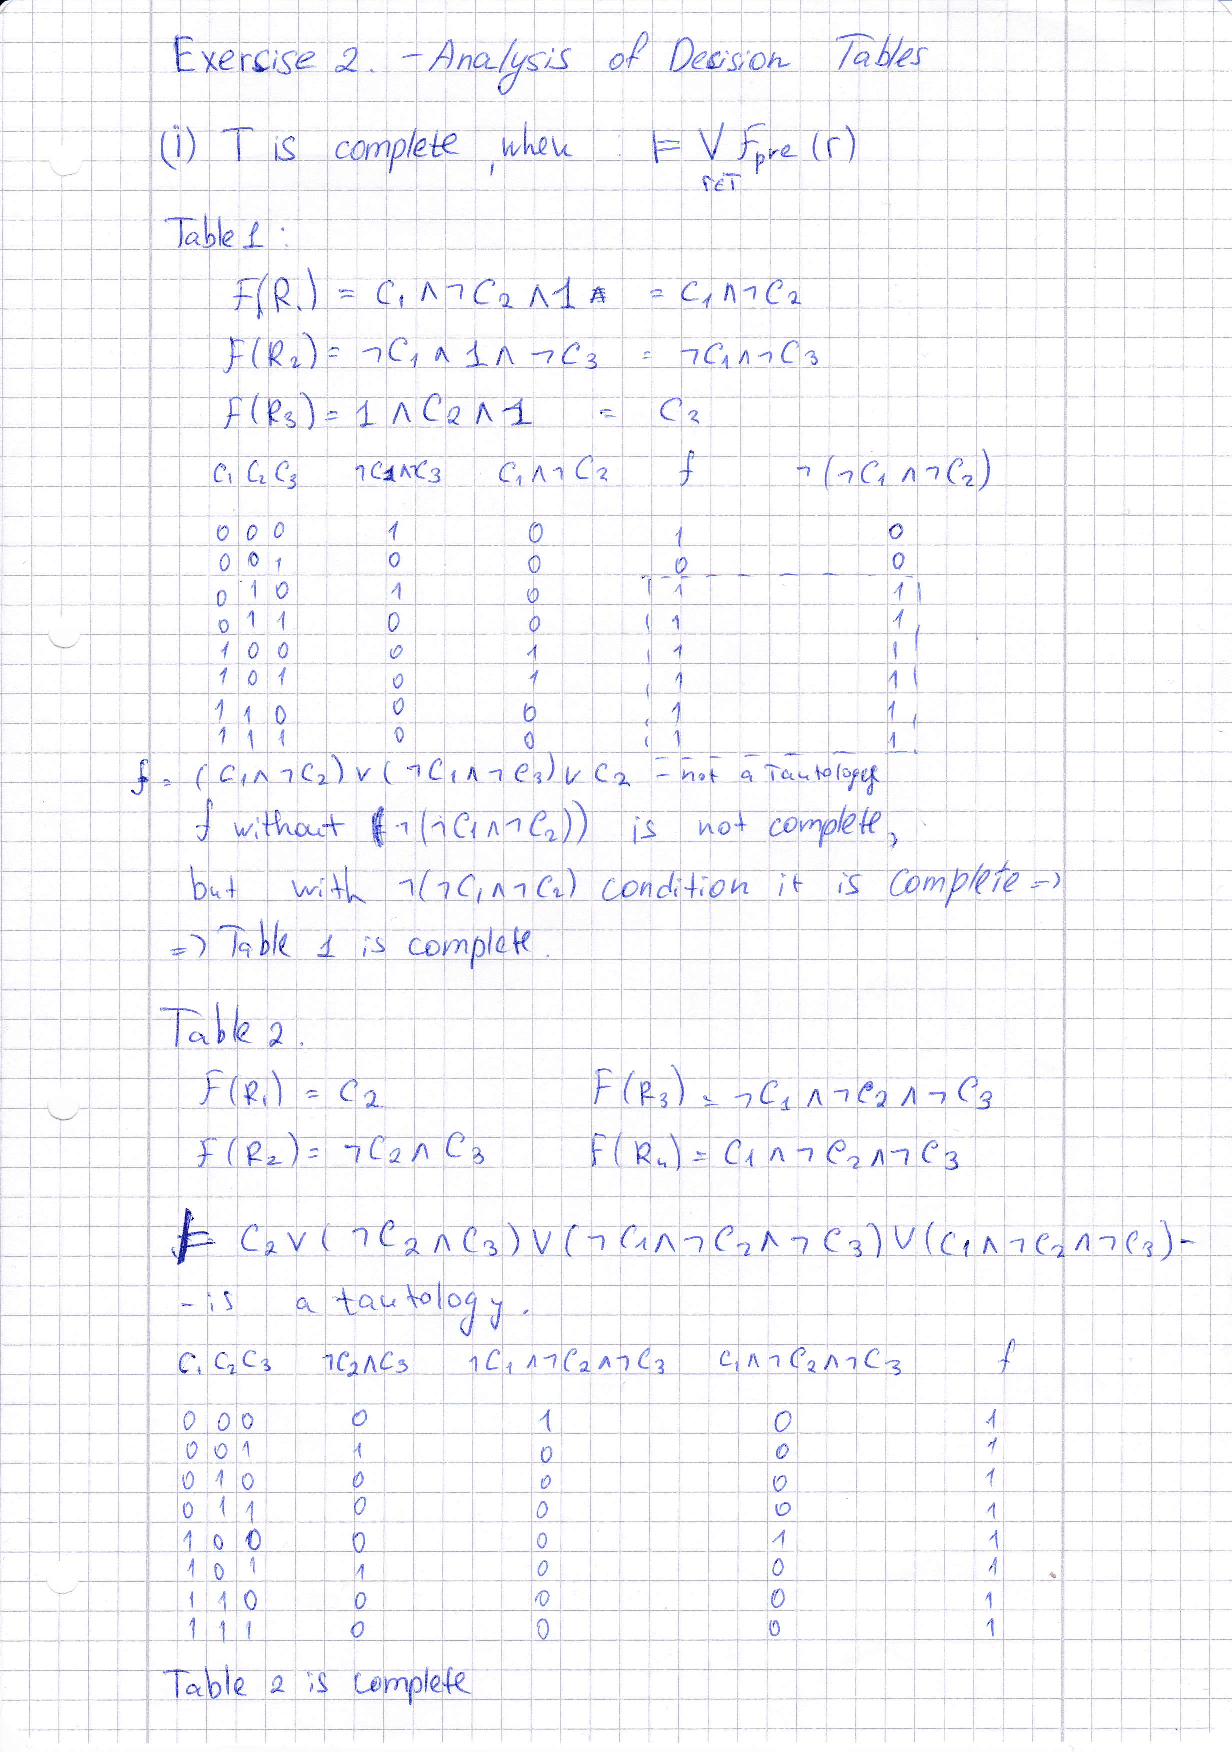
\includegraphics[scale=0.75]{Ex2a.pdf}
\newpage
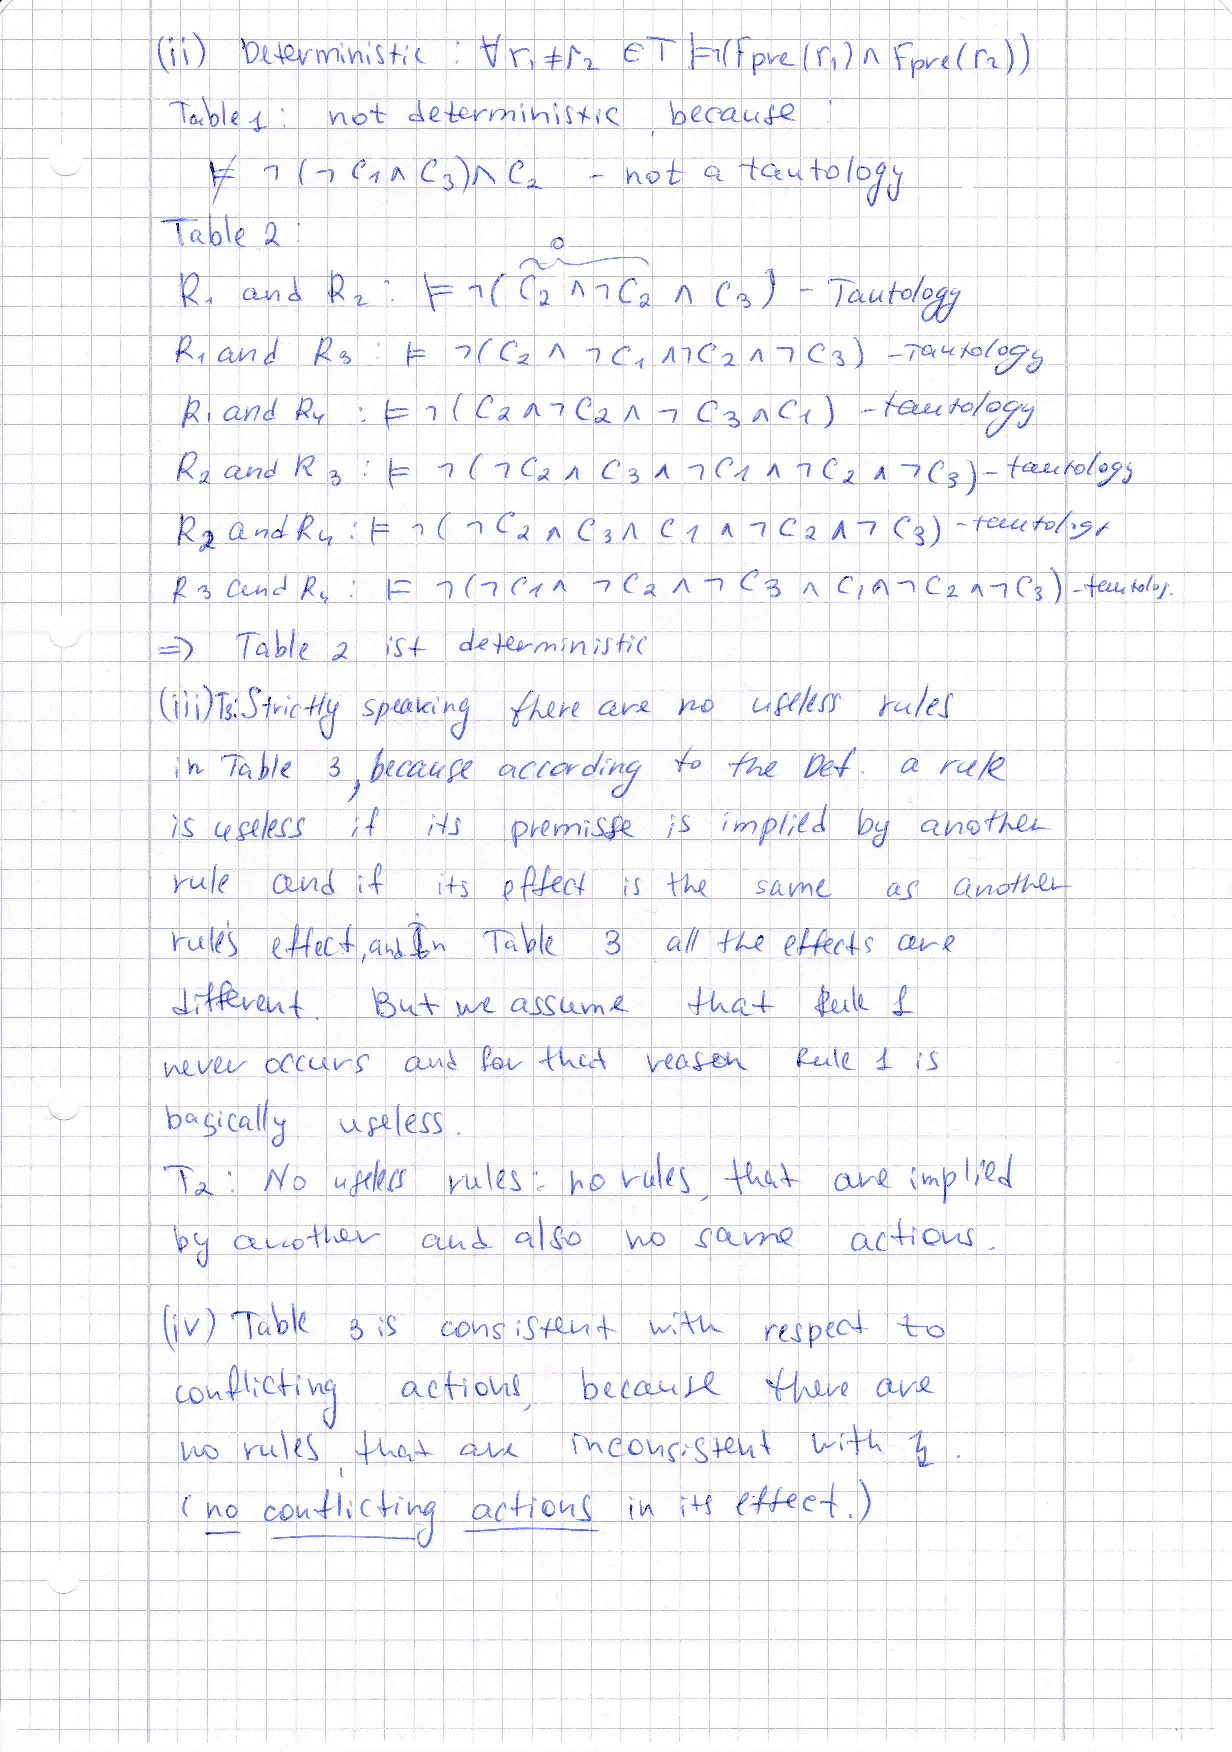
\includegraphics[scale=0.8]{Ex2b.pdf}

\subsection*{Exercise 3 – Creation of Decision Tables}

\begin{itemize}
	\item[i]
	1. For small packages, the shipping costs depend on the weight of the items in the shopping cart, there is a fixed price for the first 2kg and a variable fee for each additional kg:\\
	\begin{tabular} {l l l}
		Type & First kg. &     Additional kg.\\
		Metropolitan &     3.00 &     1\\
		Intermediate &     5 &     1.5\\
		Rural &     10.00 &     2.5
	\end{tabular}\\\\
	2. The parcel shipping costs for the first kilogram and additional kilograms are given on the following
	table:\\
	\begin{tabular} {l l l}
		Type & First kg. &     Additional kg.\\
		Metropolitan &     1.00 &     0.75\\
		Intermediate &     2.25 &     1.25\\
		Rural &     5.00 &     2.75
	\end{tabular}\\
	3. If the shipping address is in the same city as the online shop, a charge on delivery (COD) shipping option should be offered, for a fixed price of 10 Euro.\\
	4. There is a special offer: For rural areas, small but heavy packages (volumetric weight less than 5kg but more than 5kg actual weight) pay the price of intermediate cities.\\
	\begin{adjustwidth}{-4em}{-4em}
		\begin{tabular}{|p{10em} || p{2.5em} | p{3em} | p{3em} | p{3em} | p{1em} | p{3em} | p{3em} | p{3em} | p{3em} | p{4em} |}
			\hline
			DT: Price calculations & r1 (1.1)& r2 (1.2)& r3 (1.3)& r4 (4)& r5 (3)& r6 (2.1)& r7 (2.2)& r8 (2.3)\\
			\hline \hline
			effective weight $\leq$ 5kg &x&x&x&x&*&-&-&-\\
			\hline
			effective weight $>$ 5kg &-&-&-&-&*&x&x&x\\
			\hline
			metropolitan&x&-&-&-&*&x&-&-\\
			\hline
			intermediate&-&x&-&-&*&-&x&-\\
			\hline
			rural&-&-&x&x&*&-&-&x\\
			\hline
			same city as shop&*&*&*&*&x&*&*&*\\
			\hline
			actual weight $>$ 5kg &*&*&-&x&*&*&*&*\\
			\hline
			\hline
			display COD option &-&-&-&-&x&-&-&-\\
			\hline
			price calculation &3+w -1&2.25 +1.25w -1.25 &5 +2.75w -2.75&2.25 +1.25w -1.25&-&1 +0.75w -0.75&2.25 +1.25w -1.25&5 +2.75w -2.75\\
			\hline 
		\end{tabular}
	\end{adjustwidth}
	conflict axioms:\\
	The adress is either metropolitan, intermediate or rural, so no other combination (e.g $metropolitan \land rural$) cannot happen:\\
	\[
	\varphi_{confl} = ¬(metropolitan \oplus rural \oplus intermediate) \Leftrightarrow ¬(c3 \oplus c4 \oplus c5) %\equiv?
	\]
	The effective weight can be exclusively either less than or more than 5 kg:\\
	\[
	\psi_{confl} = (c1 \land c2 )\lor(¬c1 \land ¬c2)
	\]
	\item[ii]
	shipping to the \textbf{rural} area Niederaichbach, (so \textbf{not in the same city} where the shop is located) with the dimensions 29.7cm × 21cm × 20cm and a weight of 6.25kg gives us an effective weight of 5,9896 kg (\textbf{> 5 kg}) (a small package).\\
	So we can only use the rule \textbf{r4}, which give us a price of $2.25\cdot 1.25 \cdot 5.9896 -1.25\approx8.49€$
	\item[iii]
	The requirements for the text are not consistent/free from contradictions:\\The points three and four would be in conflict with the ninth point if one does not assume that they are only valid for small packages.\\\\
	The table is consistent because the interpreting function is a tautology, it has a rule for every possible combination of conditions:\\
	\begin{align*}
	&c1 \land ¬c2 \land c3 \land ¬c4 \land ¬c5 \land true \land true\\
	&\lor c1 \land ¬c2 \land ¬c3 \land c4 \land ¬c5 \land true \land true\\
	&\lor c1 \land ¬c2 \land ¬c3 \land ¬c4 \land c5 \land true \land ¬c7\\
	&\lor c1 \land ¬c2 \land ¬c3 \land ¬c4 \land c5 \land true \land c7\\
	&\lor ¬c1 \land c2 \land c3 \land ¬c4 \land ¬c5 \land true \land true\\
	&\lor ¬c1 \land c2 \land ¬c3 \land c4 \land ¬c5 \land true \land true\\
	&\lor ¬c1 \land c2 \land ¬c3 \land ¬c4 \land c5 \land true \land true\\
	&\lor true \land true \land true \land true \land true \land c6 \land true\\
	&\lor ¬(c3 \oplus c4 \oplus c5)\\
	&\lor (c1 \land c2 )\lor(¬c1 \land ¬c2)\\\\
	% \equiv ?
	&\Leftrightarrow ¬c2 \land c3 \land ¬c4 \land ¬c5\\
	&\lor ¬c2 \land ¬c3 \land c4 \land ¬c5 \\
	&\lor ¬c2 \land ¬c3 \land ¬c4 \land c5 \land ¬c7\\
	&\lor ¬c2 \land ¬c3 \land ¬c4 \land c5 \land c7\\
	&\lor c2 \land c3 \land ¬c4 \land ¬c5 \\
	&\lor c2 \land ¬c3 \land c4 \land ¬c5 \\
	&\lor c2 \land ¬c3 \land ¬c4 \land c5 \\
	&\lor c6\\
	&\lor ¬(c3 \oplus c4 \oplus c5)\\
	&\lor (c1 \land c2 )\lor(¬c1 \land ¬c2)\\
	% \equiv ?
	\end{align*}
	\newpage
	\begin{align*}
	&\Leftrightarrow ¬c2 \land c3 \land ¬c4 \land ¬c5\\
	&\lor ¬c2 \land ¬c3 \land c4 \land ¬c5 \\
	&\lor ¬c2 \land ¬c3 \land ¬c4 \land c5 \land true\\
	&\lor c2 \land c3 \land ¬c4 \land ¬c5 \\
	&\lor c2 \land ¬c3 \land c4 \land ¬c5 \\
	&\lor c2 \land ¬c3 \land ¬c4 \land c5 \\
	&\lor c6\\
	&\lor ¬(c3 \oplus c4 \oplus c5)\\
	&\lor (c1 \land c2 )\lor(¬c1 \land ¬c2)\\\\
	% \equiv ?
	&\Leftrightarrow ¬c2 \land c3 \land ¬c4 \land ¬c5\\
	&\lor ¬c2 \land ¬c3 \land c4 \land ¬c5 \\
	&\lor ¬c2 \land ¬c3 \land ¬c4 \land c5 \\
	&\lor c2 \land c3 \land ¬c4 \land ¬c5 \\
	&\lor c2 \land ¬c3 \land c4 \land ¬c5 \\
	&\lor c2 \land ¬c3 \land ¬c4 \land c5 \\
	&\lor c6\\
	&\lor ¬(c3 \oplus c4 \oplus c5)\\
	&\lor (c1 \land c2 )\lor(¬c1 \land ¬c2)\\
	\end{align*}
	because of $\psi_{confl}$ (and common sense) we can conclude that $c1 = ¬c2$ and get rid of the first (or second) row in the table ($c1$ or $c2$ in the interpreting function). The third and the fourth line differ in only one variable, so can be reduced to one line without $c7$.\\
\end{itemize}

\subsection*{Exercise 4 – Use Cases}

\begin{itemize}
    \item[i]
        \begin{tabular}{|l|l|}
            \hline
            name            & Chack Balance \\ \hline
            goal            & Show specific information about the latest transactions \\ \hline
            pre-condition   & User Authenticated, showing Main Menu, ATM is operational \\ \hline
            post-condition  & showing Main Menu, Maybe printed Summary \\ \hline
            post-condition  & withholding/returning card \\
            in exception-case & and return to authentication screen \\ \hline
            actors          & client (main actor), bank system, printer\\ \hline
            open questions  & none \\ \hline
            normal case     & 1. User Presses 'Balance'-Button \\
                            & 2. get balance-information from bank-system \\
                            & 3. ATM shows Balance-Summary screen \\
                            & 4. User presses confirm \\
                            & 5. returns to Main screen \\ \hline
            normal case 2   & 1. User Presses 'Balance'-Button \\
                            & 2. get balance-information from bank-system \\
                            & 3. ATM shows balance-summary screen \\
                            & 4. User presses print-button \\
                            & 5. disable print-button \\
                            & 6. balance summary will be printed \\
                            & 7. Success-Message appears on screen \\
                            & 8. User pushes confirm button \\
                            & 9. returns to Main screen \\ \hline
            exc. case 0a    & User not responding for 30sec \\
                            & 0.1 withhold card \\
                            & 0.2 return to authentication screen \\ \hline
            exc. case 0b    & Weird sensory data \\
                            & 0b.1 withhold card \\
                            & 0b.2 return to authentication screen \\ \hline
            exc. case 2a    & No connection to bank system could be established \\
                            & 2a.1 show error message \\
                            & 2a.2 show Authentication screen \\
                            & 2a.3 return card \\ \hline
            exc. case 6a    & Printer cannot print \\
                            & 6a.1 Message about not workign printer appears on screen \\
                            & 6a.2 (continue with default point 8) \\ \hline

        \end{tabular}
    \item[ii]
    	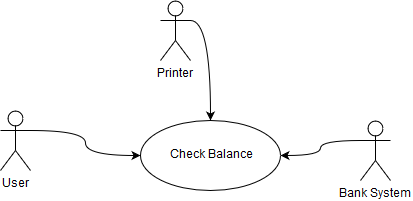
\includegraphics[width=8cm]{use_case_diagram.png} \\
        This use-case diagram only contains the use-case names and the actors.
\end{itemize}

\end{document}
